% Options for packages loaded elsewhere
\PassOptionsToPackage{unicode}{hyperref}
\PassOptionsToPackage{hyphens}{url}
%
\documentclass[
  12pt,
]{book}
\usepackage{amsmath,amssymb}
\usepackage[]{libertinus}
\usepackage{setspace}
\usepackage{iftex}
\ifPDFTeX
  \usepackage[T1]{fontenc}
  \usepackage[utf8]{inputenc}
  \usepackage{textcomp} % provide euro and other symbols
\else % if luatex or xetex
  \usepackage{unicode-math}
  \defaultfontfeatures{Scale=MatchLowercase}
  \defaultfontfeatures[\rmfamily]{Ligatures=TeX,Scale=1}
\fi
% Use upquote if available, for straight quotes in verbatim environments
\IfFileExists{upquote.sty}{\usepackage{upquote}}{}
\IfFileExists{microtype.sty}{% use microtype if available
  \usepackage[]{microtype}
  \UseMicrotypeSet[protrusion]{basicmath} % disable protrusion for tt fonts
}{}
\makeatletter
\@ifundefined{KOMAClassName}{% if non-KOMA class
  \IfFileExists{parskip.sty}{%
    \usepackage{parskip}
  }{% else
    \setlength{\parindent}{0pt}
    \setlength{\parskip}{6pt plus 2pt minus 1pt}}
}{% if KOMA class
  \KOMAoptions{parskip=half}}
\makeatother
\usepackage{xcolor}
\IfFileExists{xurl.sty}{\usepackage{xurl}}{} % add URL line breaks if available
\IfFileExists{bookmark.sty}{\usepackage{bookmark}}{\usepackage{hyperref}}
\hypersetup{
  pdftitle={Marc Nickl},
  hidelinks,
  pdfcreator={LaTeX via pandoc}}
\urlstyle{same} % disable monospaced font for URLs
\usepackage[a4paper,margin=1in]{geometry}
\usepackage{graphicx}
\makeatletter
\def\maxwidth{\ifdim\Gin@nat@width>\linewidth\linewidth\else\Gin@nat@width\fi}
\def\maxheight{\ifdim\Gin@nat@height>\textheight\textheight\else\Gin@nat@height\fi}
\makeatother
% Scale images if necessary, so that they will not overflow the page
% margins by default, and it is still possible to overwrite the defaults
% using explicit options in \includegraphics[width, height, ...]{}
\setkeys{Gin}{width=\maxwidth,height=\maxheight,keepaspectratio}
% Set default figure placement to htbp
\makeatletter
\def\fps@figure{htbp}
\makeatother
\setlength{\emergencystretch}{3em} % prevent overfull lines
\providecommand{\tightlist}{%
  \setlength{\itemsep}{0pt}\setlength{\parskip}{0pt}}
\setcounter{secnumdepth}{-\maxdimen} % remove section numbering
\newlength{\cslhangindent}
\setlength{\cslhangindent}{1.5em}
\newlength{\csllabelwidth}
\setlength{\csllabelwidth}{3em}
\newlength{\cslentryspacingunit} % times entry-spacing
\setlength{\cslentryspacingunit}{\parskip}
\newenvironment{CSLReferences}[2] % #1 hanging-ident, #2 entry spacing
 {% don't indent paragraphs
  \setlength{\parindent}{0pt}
  % turn on hanging indent if param 1 is 1
  \ifodd #1
  \let\oldpar\par
  \def\par{\hangindent=\cslhangindent\oldpar}
  \fi
  % set entry spacing
  \setlength{\parskip}{#2\cslentryspacingunit}
 }%
 {}
\usepackage{calc}
\newcommand{\CSLBlock}[1]{#1\hfill\break}
\newcommand{\CSLLeftMargin}[1]{\parbox[t]{\csllabelwidth}{#1}}
\newcommand{\CSLRightInline}[1]{\parbox[t]{\linewidth - \csllabelwidth}{#1}\break}
\newcommand{\CSLIndent}[1]{\hspace{\cslhangindent}#1}
\usepackage{graphicx}
\usepackage{multibib}
\ifLuaTeX
  \usepackage{selnolig}  % disable illegal ligatures
\fi

\author{}
\date{}

\begin{document}
\frontmatter

\listoffigures
\setstretch{1.5}
\mainmatter
\pagenumbering{arabic}

\begin{titlepage}
    \begin{center}
        \vspace*{4cm}
            
  \LARGE
        \textbf{Herzog and Broomfield}
            
 \vspace{0.5cm}
        \Large
        Compare the non-fiction work of any two directors referenced within this unit
            
   \vspace{10cm}
            
\textbf{Marc Nickl}
            
\vfill
            
            
 \vspace{0.8cm}
                        
   \large
        Screen Studies 
        
\today
            
 \end{center}
\end{titlepage}

\setcounter{tocdepth}{3}
\tableofcontents
\pagebreak

\vspace{20pt}

\begin{center}
“An endless struggle with great benefits of satisfaction when you get to the end” (Broomfield, 2017)

\end{center}

\vspace{20pt}

\hypertarget{title}{%
\section{Title}\label{title}}

\hypertarget{subtitle}{%
\subsection{Subtitle}\label{subtitle}}

\hypertarget{one-below-that}{%
\subsubsection{one below that}\label{one-below-that}}

\hypertarget{another-one}{%
\paragraph{another one}\label{another-one}}

\emph{italics} \textbf{bold} 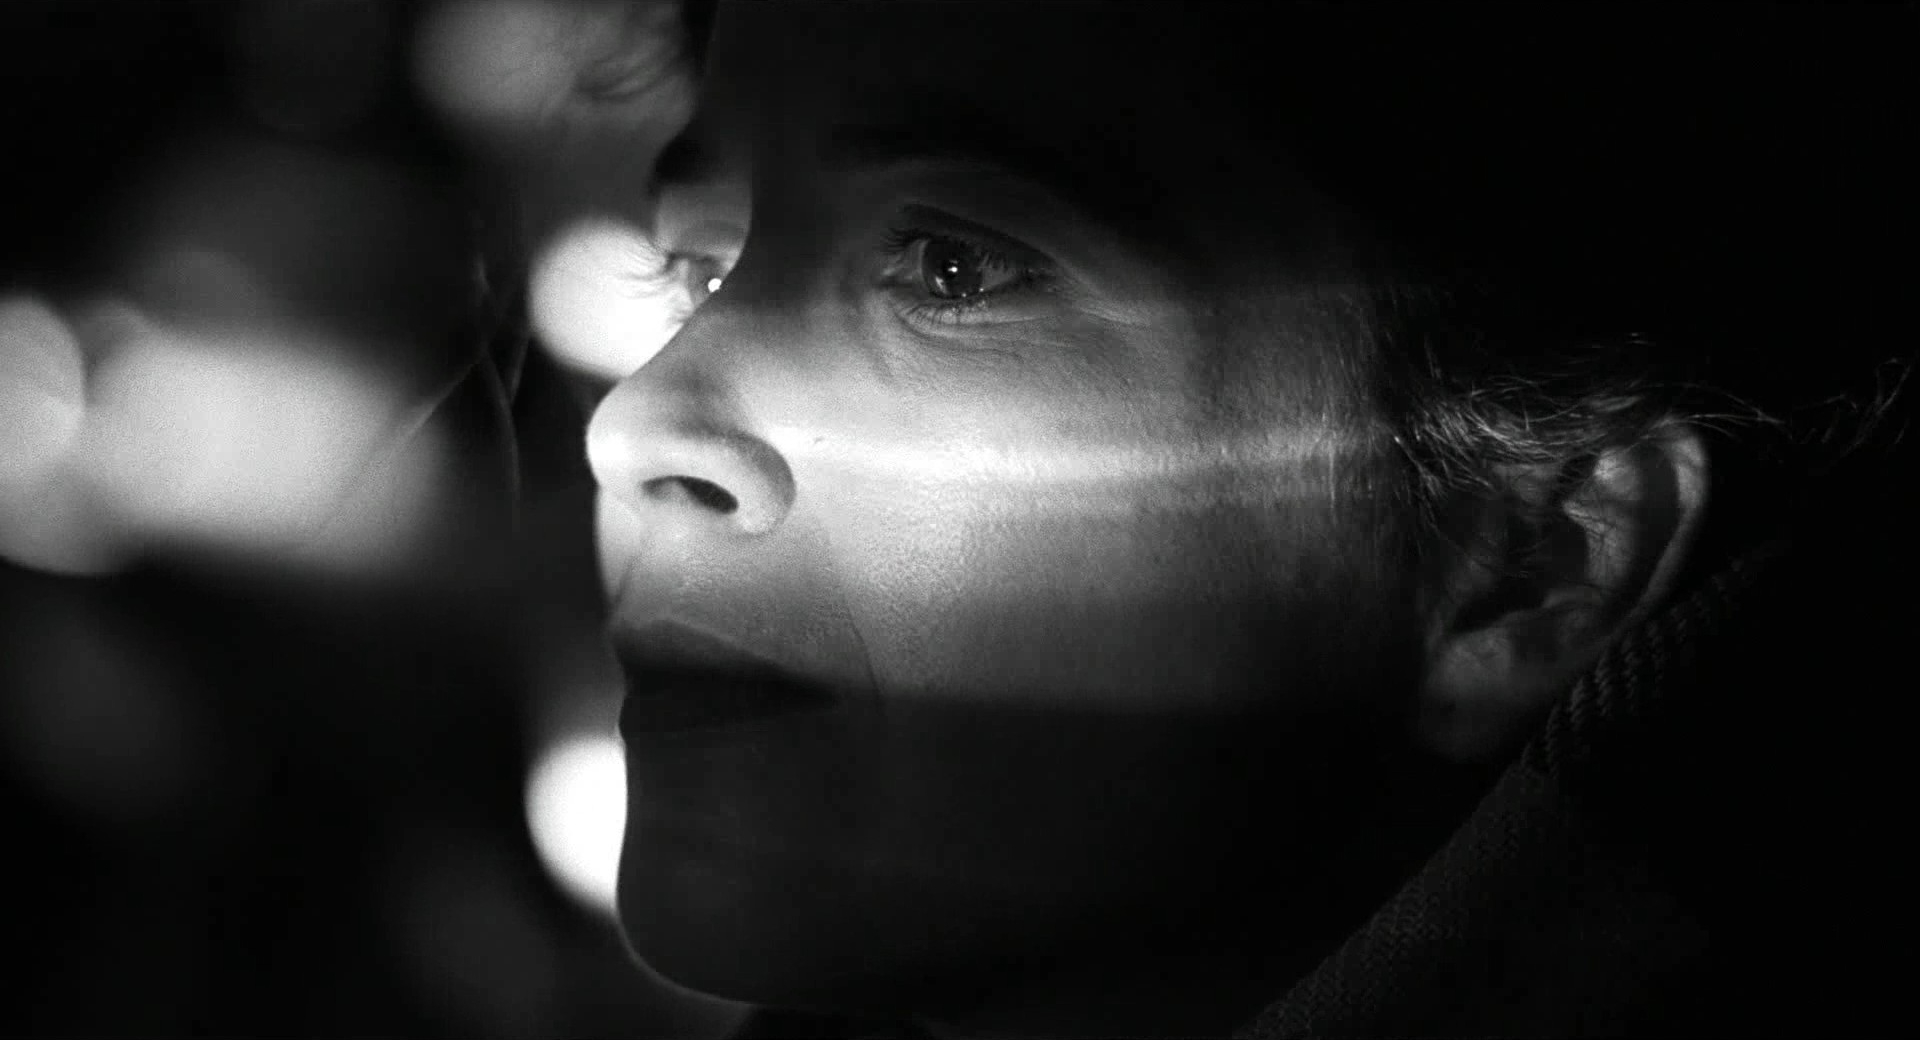
\includegraphics{0314b786c05d34aa190fcc8bf3c6696c.png}

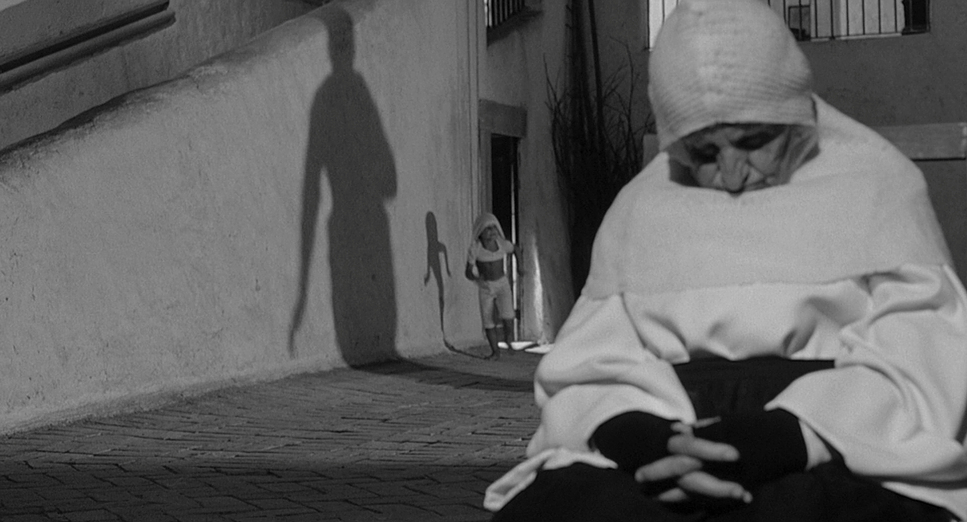
\includegraphics{fd4fef9a20383db8ff25d8806505b409.png} \# This sis for fun

\begin{figure}[ht]

\centering

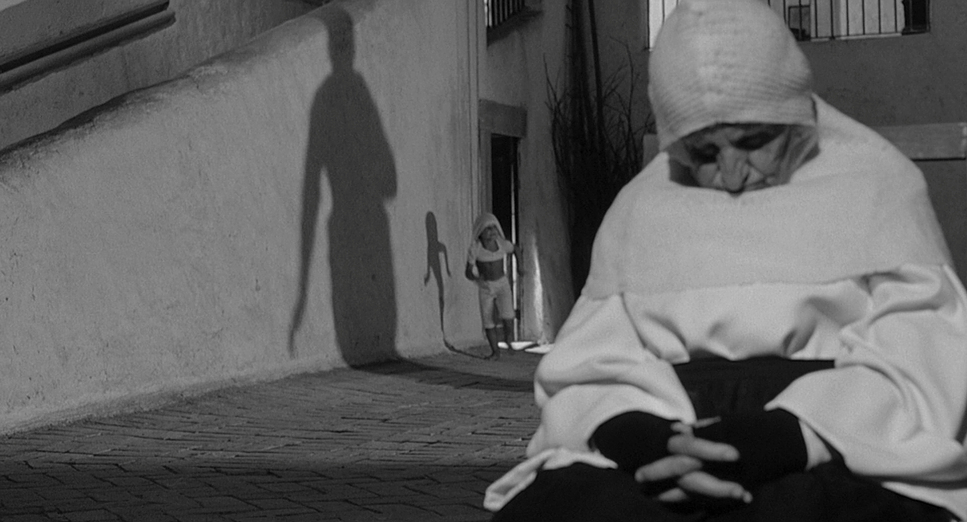
\includegraphics[width=\linewidth]{fd4fef9a20383db8ff25d8806505b409.png}

\caption[Short Title]{\textbf{Short Title:} A long description of the image}

\label{fig:foo}

\end{figure}

This is a sub heading this is the main body of the text

(\textbf{noauthor\_2014-nk?}) 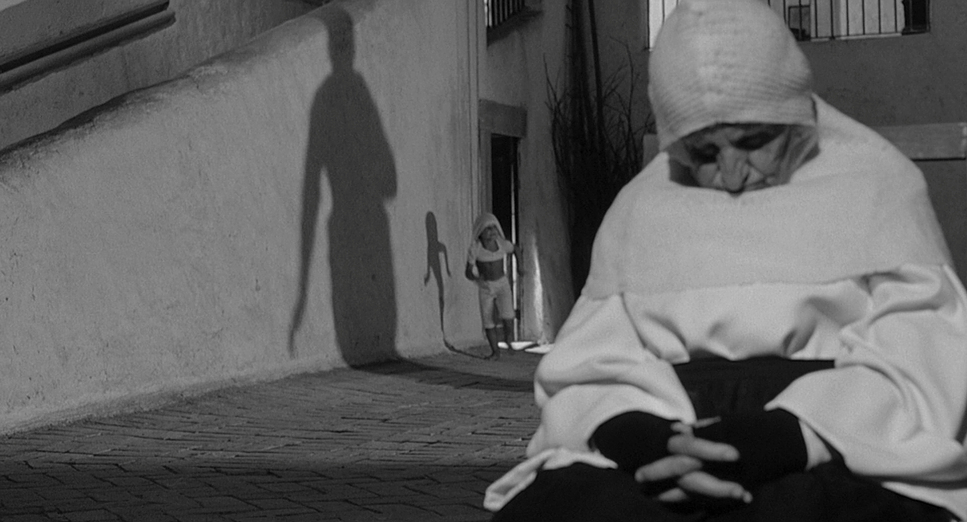
\includegraphics{fd4fef9a20383db8ff25d8806505b409.png}

\textrm{lol }\\
\textsf{ment to be serif }\\
\texttt{text }\\
\textmd{text }\\
\textbf{text }\\
\textup{also not sure }\\
\textit{even less of a clue }\\
\textsl{less clue }\\
\textsc{dont know }\\
\emph{this is an emphasis }\\
\textnormal{text}\{\textbackslash normalfont text\}Document font

\underline{this is underlined }

actors to recreate scenes and Werner Herzog's use of scripting interviews in Lessons in Darkness (2001), where he has ``frontal shots of war victims delivering scripted poetic monologues'' (\textbf{Peucker2012-px?})

In this essay I am going to compare the non-fiction work of Werner Herzog and Nick Broomfield, both highly distinguished filmmakers. The essay has the goal of getting a greater understanding of how their work has evolved over the span of their long, unique and inspiring careers. I will compare their work in a number of ways. First I'll be looking at how their beginnings might have influenced them as filmmakers. Then I will look at how their style of filming and the means by which they convey truth and reality to the audience has evolved over the years. The final aspect I will look at is how both Directors approach the same subject matter. Here I intend to look at the film (Aileen: Life and Death of a Serial Killer, 2003) by Nick Broomfield and Into the Abyss, (2012) by Werner Herzog. Both films look at the crime and execution of a serial killer, having interviews with the convicts just a few days before they were to die.

Nick Broomfield's journey in film started when he was studying political science at the University of Essex and law at the University College Cardiff. He borrowed a film camera from the rugby club at the University College Cardiff which he then used to make his first film in Liverpool about the problems of slum demolition and the removal of residents to new housing blocks. The film is called Who Cares (Who Cares, 1971). This led to him joining the National Film and Television School in 1973, which is where he met the cinematographer and his lifelong collaborator Joan Churchill.

Ten years earlier Werner Herzog had started his film career by reading ``an encyclopedia, the fifteen or so pages on filmmaking. Everything I needed to get myself started came from this book.'' (Cronin and Herzog, 2003:28) This led to him stealing a 35mm film camera from the Munich Film School, which made it possible for him to make his first film (Herakles, 1962) about competitive bodybuilders. Two year later he started work on the film Spiel im Sand, 1964, however it was never released as ``things were moving out of control'' (Cronin and Herzog, 2003). He continued to make short documentaries till 1970 when he made The Flying Doctors of East Africa.

Being self taught, Herzog had a unique and personal style and the artform of his work has always stood out as being very individual. Throughout the span of Herzog's career, his sensibilities have not changed, although you can see improvements in his film craft.

In the careers of both Herzog and Broomfield, you see the greatest differences in directorial style in the first films they did. The films are polar opposites in the way they are shot and cut together. Who Cares, (1971) is a more personal film in many ways, following a subject matter that Nick Broomfield cared about and taking over a year to cut. ``I had a strong feeling making this film that modernity has destroyed so much of people's sense of belonging'' (Who Cares - Nick Broomfield's Official Website, s.d.) This is clearly seen in the film where each shot, each cut seems purposeful, holding shots where needed and creating a steady decisive look. Generally it feels more mature for a first film.

Compare this to the film Herakles, which has closer ties to earlier montage cinema, inter-cutting between bodybuilders preparing for competition with stock footage of disaster, like the crash at Le Mans in 1955, or post world war two clean up. This creates a faster cutting pace and it seems like a less thought out cut. In Herzog's own words, ``My most immediate and radical lesson came from what was my first blunder, Herakles'' (Cronin and Herzog, 2003:24).

When talking about the style of a filmmaker an important question is. - Where did the style come from and if it evolved why?

As Nick Broomfield studied at the National Film School a connection can be made that the style of his early works like Proud to Be British, 1973 or Juvenile Liaison,1976 were hugely influenced by the popular documentary style at the time, cinéma vérité, and therefore by the tutelage of Colin Young, the founding director of the NFTS. Young was at the time writing the manifesto-essay titled Observational Cinema, published in Principles of Visual Anthropology (Young and Hockings, 1975:99). In the essay he states that, ``The difference is between TELLING a story and SHOWING us something'' is completely different. This is one of the key principles of cinéma vérite, where the film attempts to show reality without the influence of the storyteller. He also states that, ``\ldots we are spending time perfecting our ability to see straight, shoot straight, and edit the sections so that the parts of our film have a sense of the whole,\ldots{}''(Young and Hockings, 1975:112)

Another point regarding the question of nature or nurture in filmmakers is when Nick Broomfield's collaboration with Joan Churchill comes to an end in the late 1980's. There is a clear change in style in Broomfield's work. His approach to documentaries changed from the aforementioned Cinéma Vérité to his pioneering on-screen appearance with Participatory Documentary in Driving Me Crazy (1988). This was due to the production of Driving Me Crazy going ``hopelessly out of control.'' (Fairweather, 2007).

Fig 1 Nick Broomfield's first appearance on camera

Fig 2 Nick Broomfield on the left

Broomfield made a deal with his producers that he would only continue to work on the film if he could film everything surrounding the production, including the conversations behind the scenes. This gave him the opportunity to experiment. In an interview with Aesthetica he said, ``It enables you to establish a more in-depth relationship with people. When filming you show more things than in a feature film, which requires a beginning, middle and end sequence. Appearing in the film gives you the flexibility to include thoughts and flashing of things, contextualising what is happening.'' (Fairweather, 2007) He continues to say, ``The thing that excites me about filmmaking is the spontaneity, I want there to be energy, so that it feels real.'' (Fairweather, 2007) This change in style has remained till the present day (with a few exceptions).

Fig 3 Werner Herzog's first appearance on camera

Werner Herzog is more known for his presence on screen and for appearing in front of the camera. Similar to Nick Broomfield's first time, he did not appear in front of the camera of his own volition, but because he was ``forced to make an appearance''. (Cronin and Herzog, 2003:180) This was due to (Die große Ekstase des Bildschnitzers Steiner, 1974) being produced in a series called Grenzstationen, where it was stipulated that Herzog had to ``conform to the network's rules, one of which was that the filmmaker had to appear in the film as the chronicler of events'' (Cronin and Herzog, 2003:180). Herzog said himself about this, that, ``Some people look at a film like The Great Ecstasy of Woodcarver Steiner and accuse me of self-promotion because I appear in the film.'' However, as said, this was a requirement from the producers. Nevertheless, like with Broomfield, it was due to this experience of appearing in front of camera that he realised the possibilities and potential of this style of filming. Since The Great Ecstasy of Woodcarver Steiner (1974) Herzog has appeared in all of his documentary films in one form or another. Poetic Truth and Direct Cinema

Both filmmakers have also carved out their own styles in documentary cinema. Their `rebellious' alteration from the norms can be seen in both Nick Broomfield's use of actors to recreate scenes and Werner Herzog's use of scripting interviews in Lessons in Darkness (2001), where he has ``frontal shots of war victims delivering scripted poetic monologues'' (Peucker, 2012:37). He describes it as `ecstatic truth'; ``what moves me has never been reality, but a question that lies behind it {[}beyond; dahinter{]}: the question of truth. Sometimes facts so exceed our expectations---have such an unusual, bizarre power---that they seem unbelievable.'' (Herzog and Weigel, 2010:8--9).

There is a fine line between reality and fiction and both Nick Broomfield and Werner Herzog have teetered on the edge, where the boundary becomes a bit smudged. This creates a dilemma for anyone trying to categorise where a film belongs, it can also be a weird line to go down when trying to make a film where one wants the viewer to feel something, whether that be a sense of truth or just simple excitement.

``Through invention, through imagination, through fabrication, I become more truthful than the little bureaucrats.'' (Cronin and Herzog, 2003:240), One of the key things that makes Werner Herzog and his work stand out since the very beginning is their originality as he advocates for a more poetic interpretation of truth in documentary filmmaking, sometimes blurring the lines between reality and fiction - ``my non-fiction films are pretty much fiction, or at least close.'' (Herzog, 2007) He often ``played with the `truth' of the situation to reach a more poetic understanding'' (Cronin and Herzog, 2003:253). This might have come from his self-taught upbringing in film.

Although a work of fiction, Fitzcarraldo (1982) is a perfect example of where the lines get blurred and the film ends up on the fiction side of the spectrum. Herzog has taken much more liberty with facts and actual happenings in weaving together a story for his films.

\begin{quote}
The closest that Nick Broomfield comes to this is in Ghosts. “The later films of Nick Broomfield take this notion of constructed truth a stage further as they build themselves around the encounters between subjects and Broomfield’s on-screen alter ego … on the nature of documentary authenticity.”     
\end{quote}

(\textbf{Bruzzi2006-uy?})

In Ghosts (2006) we see the final alteration in Nick Broomfield's style, which he directed in 2006. This is a story about the immigration of a Chinese national to the UK who came hoping to earn an income so that she could support her family back in China. She gets an underpaid job in a UK meat packing factory. The film recreates the Morecambe Bay cockling disaster where she and 22 other illegal workers drowned picking cockles (Bradshaw, 2007). \ldots{} Ghosts closely follows the style of what he calls ``Direct Cinema'', meaning that he used actors to recreate the story.

There is a lot of noise and opposing opinions on what the term `Direct Cinema' means. The `more common' academic definitions are slightly different from Broomfield's interpretation. The academic difference between Cinéma Vérité and Direct Cinema is that ``Cinéma vérité wanted to explain the raison d'être of life, whereas Direct Cinema wanted to let life reveal itself'' (McLane, 2012). However, Broomfield ``calls ``direct cinema'' also known as ``enhanced reality'', where non-actors play themselves in scripted dialogue.'' (Williams, 2017) This definition better covers what Broomfield has stylistically done in Ghosts (2006) and Battle for Haditha (2007) where he uses actors to recreate scenes that would otherwise not have been shot.

Whilst this style of filming is on the edge of what I would consider a documentary, due to its use of non-actors, I do think this is where Broomfield and Herzog are closest stylistically. Although Herzog hasn't made direct use of recreation or reenactment, he was the executive producer on The Act of Killing (2012) which uses both to great effect.

Comparing two films To gain a closer insight into the styles of two filmmakers, one needs to look at their production of films having the same subject matter. This is rarely possible, however, in the case of Nick Broomfield and Werner Herzog, it is possible. Both of them made films about murderers who were on death row, including interviews with the convicts in their last days. Aileen: Life and Death of a Serial Killer (2003) by Nick Broomfield and Into the Abyss (2011) by Werner Herzog.

Aileen: Life and Death of a Serial Killer (2003), is the second part of the Aileen Wuornos story. The first part happened 10 years earlier with Aileen Wuornos: The Selling of a Serial Killer (1992). (In this film, Broomfield was again collaborating with Joan Churchill after many years apart.)

There have been many documentary and fiction films looking at the story of Aileen Wuornos, like the film by Patty Jenkins called Monster (2003). In fact, in her research for the role of Aileen, Charlize Theron, who was to play that role, asked Nick Broomfield, who at the time was shooting the second Aileen Wuornos documentary film, for footage which she could use as character reference. Nick Broomfield sent `` them a rough cut of the second film'' (Wood, 2005:62).

In Nick Broomfield's autobiography he was asked by Jason Wood, ``Nearly all the articles on Monster deflected attention back to your films'', to which he responded with ``I had the choice of either working with them and trying to make it into a positive experience that would help both films and an understanding of Aileen {[}or not{]}\ldots{} I think we actually did benefit from each other and, in a way, the films authenticated Charlize's performance. The films fed off each other.''(Wood, 2005:62--63) In spite of being a documentary, the critics have stated that the film by Nick Broomfield had more drama than the fictional work of Patty Jenkins. This goes to show the power of a good story when brought to life in a documentary well made. ``In the end, Broomfield and Churchill's search for truth inevitably trumps Jenkins's fictionalisation. Even Theron's remarkable acting\ldots. is superseded by Broomfield's interview with Wuornos on the eve of her execution.'' (Patterson, 2004)

Werner Herzog's film on this subject matter is Into The Abyss: A Tale of Death, a Tale Of Life (2012). The film follows the life and death of Michael Perry who was sentenced to death row for the murder of three people.\\
The film documents the tragic story of Michael Perry and his friend Jason Burkett, two drugged-up teenagers, coming from a deprived background, who decide to steal a red sports car from an affluent gated community. In the process they kill three people, have the car for seventy two hours before being pursued by the police and arrested and consequently sentenced.

To make this film, Herzog uses archive footage and interviews with friends, family and police, concluding with an interview with the convict shortly before his death. Into The Abyss only had 4 hours of shoot footage out of which Herzog masterfully creates a film so moving and shocking \ldots{}

(Compare this to Aileen, where there was an immense amount of footage as Broomfield had followed and even taken part in the proceedings.)

The quote by Nietzsche in his book Beyond Good and Evil, perfectly describes Herzog's film, Into The Abyss; ``when you look for a long time into an abyss, the abyss also looks into you.'' (Nietzsche, 1886). In an interview, Herzog himself said of this film that ``it allows us looking into the abyss'' (Herzog, 2012).

, \{often for those living on death row documentary on Aileen Wuornos by Nick Broomfield and Werner Herzog's Into the

Through both films God is referenced a lot, this could either be a point to look at however I don't know how both filmmakers react to it

Society failed both convicts and they in turn,

Conclusion to the direct comparison In their works on death row both Werner Herzog and Nick Broomfield have been described as ``offering an account of the convicted humanity\ldots in a society obsessed with victim culture.'' (Picart et al., 2016:245) in Framing Law and Crime: An Interdisciplinary Anthology. This makes watching the films even more emotionally taxing as you begin to relate to the characters portrayed in them, even to the point of feeling sympathy for them. The two filmmakers both have a certain level of sensitivity and humanity when filming these characters, although disagreeing with their actions, still treating them like humans.

The documentaries do not shy away from revealing the authors' clear objections to sentencing people to the death penalty. ``Herzog (who has made clear in interviews that he believes no state should put a human being to death) sets out to raise the question in a manner at once precise, poignant, and mindful of complexity, through the investigation of a horrific story and its consequences.'' (Biles, 2012:2) Broomfield said on this subject, ``The violence of taking a life remains the same whether it is legally sanctioned or not. lt introduces murder into our vocabulary of behaviour.'' He also said that this was his most personal film, one that he did not choose to make but had become involved in as he was called to be a witness following his work on the earlier documentary Aileen Wuornos: The Selling of a Serial Killer (1992) and which ``ended up {[}with his{]} attending an execution'', something that had a profound and disturbing effect on him. (Aileen: The Life and Death of a Serial Killer - Nick Broomfield's Official Website, s.d.)

Wee little conclusion para This goes against the conventional style of observational cinema.

Being oneself in film is hard especially

Their influences on film/

how they've affected the filmmaking scene {[}2MN8{]} 100 words

Short paragraph on how they have influenced the filmmaking community

``Someone I've looked up to for many years, someone who represented sort of a gold standard for the kind of documentary making I aspired to do'' (Sheffield Doc Fest 2017 The BBC Interview Louis Theroux meets Nick Broomfield - YouTube, s.d.)

(Sheffield Doc Fest 2017 The BBC Interview Louis Theroux meets Nick Broomfield)

Other filmmakers using the name werner herzog to publish there documentaries

Herzog appearing in

Conclusion

Throughout their career in film, Herzog and Broomfield have used different stylistic interpretations of documentary cinema to tell a story, together they have gone from one end of the documentary spectrum to the other. They have captured `real life' as Dr.~Jeffrey Geiger referred to in a speech ``Both men's films show that real life occurs in the margins'' (Geiger, 2006). Both filmmakers are trying and also succeeding to bring the human condition to the screen, often choosing subjects who live on the outskirts of society, on the edge of social order. They have been highly inspirational to a whole generation of filmmakers and have affected the world as we know it today, opening the eyes of their viewers and raising awareness.

When a camera is put in someone's face they stop acting naturally and become self conscious. In the words of Louis Marcorelles ``I want to discover something about people. When you interview someone they always tell you what they want you to know about them'' (Marcorelles, 1973:55) and ``You don't show the whole of a subject; you select; and your selection matters'' (Marcorelles, 1973:53) Being able to direct and manipulate the footage to get some semblance of what `real' life looks like requires great skill and practice. Both filmmakers have got the ability to do exactly that.

To conclude both filmmakers are highly distinguished and respected throughout the field of filmmaking. Both peoples' films have made the world a better place. They both share a simple need to make films and both were picky about their subjects. From their early stages, where both directors had very different approaches to film, one can see how they evolve, coming ever closer, including themselves on screen and finally covering the same subject matter, even with similar ethics. So, yes, both filmmakers are different in a myriad of ways, but they still share the same values in making films.\\
(Aufderheide, 2008)

(Adobe Systems, 2003)

\pagebreak

\hypertarget{List of Figures}{%
\chapter*{List of Figures}\label{List of Figures}}
\addcontentsline{toc}{section}{List of Figures}

Figure 1. Broomfield, N. (1988) \emph{Driving Me Crazy}. {[}Still from documentary{]} At: https://www.imdb.com/title/tt0146652/?ref\_=nm\_flmg\_dr\_26

Figure 2. Herzog, W. (1974) \emph{The Great Ecstasy of Woodcarver Steiner}. {[}Still From Documentary {]} At: https://www.imdb.com/title/tt0146652/?ref\_=nv\_sr\_srsg\_4

Figure 3. Penn, Z. (2004) \emph{Incident at Loch Ness (2004)}. {[}Movie Poster{]} At: https://www.imdb.com/title/tt0374639/mediaviewer/rm3666779392/

Figure 4. Broomfield, N. (1988) \emph{Driving Me Crazy}. {[}Still from documentary{]} At: https://www.imdb.com/title/tt0146652/?ref\_=nm\_flmg\_dr\_26

\hypertarget{bibliography}{%
\chapter*{Bibliography}\label{bibliography}}
\addcontentsline{toc}{chapter}{Bibliography}

\hypertarget{refs}{}
\begin{CSLReferences}{0}{0}
\leavevmode\vadjust pre{\hypertarget{ref-adobesystemsPremierePro2003}{}}%
Adobe Systems (2003) \emph{Premiere Pro}. (s.l.): Adobe.

\leavevmode\vadjust pre{\hypertarget{ref-aufderheideDocumentaryFilmVery2008}{}}%
Aufderheide, P. (2008) \emph{Documentary Film: A Very Short Introduction}. New York: OUP USA.

\end{CSLReferences}

\backmatter
\end{document}
